\chapter{Diversité des organismes unicellulaires}\label{ch:b2:unicellular-diversity}

Une goutte d'eau de mare sous le microscope contient une cellule verte
qui rame avec deux flagelles, un cilié en forme de pantoufle qui balaie
des bactéries vers son cytopharynx, une diatomée vitreuse qui glisse sur
la lame et, trop petites pour être bien vues, un millier de bactéries.
Chacune est une seule cellule et chacune est un organisme entier~: elle
se nourrit, se déplace, perçoit, croît, se reproduit et meurt en tant
que cellule unique. La plus grande partie du monde vivant a toujours été
ainsi. Ce chapitre traite l'\omterm{def:b2:unicellular-diversity:unicellular}{organisme unicellulaire} comme un problème de
conception --- ce qu'une cellule peut faire et ne peut pas faire --- et
passe en revue les réponses qu'ont trouvées les \omterm{def:b2:unicellular-diversity:prokaryote}{procaryotes} et les
eucaryotes, jusqu'au point où les cellules commencent à rester ensemble.

\section{Une cellule, toutes les fonctions}

\begin{definition}[Unicellulaire, colonial, pluricellulaire]\label{def:b2:unicellular-diversity:unicellular}
Un organisme est \emph{unicellulaire}\index{organisme unicellulaire} lorsqu'une
seule cellule assure toutes les fonctions de la vie --- nutrition,
échanges, mouvement, reproduction --- et vit par elle-même. Il est
\emph{colonial}\index{organisme colonial} lorsque des cellules d'un même
type restent attachées après la division, chacune restant capable de
vivre seule si on l'isole. Il est \emph{pluricellulaire}\index{organisme pluricellulaire}
lorsque ses cellules sont de plusieurs types, dépendent les unes des
autres, et que quelques-unes seulement (la lignée germinale) laissent
une descendance. Les organismes unicellulaires comprennent toutes les
archées, presque toutes les bactéries et la plupart des lignées
d'eucaryotes~; le nom informel de \emph{\omterm{def:b2:unicellular-diversity:protist}{protiste}} désigne les
eucaryotes unicellulaires, qui ne forment pas un groupe mais plusieurs.
\end{definition}

\begin{example}[Six habitants d'une goutte]\label{ex:b2:unicellular-diversity:drop}
\emph{Escherichia coli}, un bâtonnet long de \qty{2}{\micro m}, nage
grâce à une touffe de flagelles et se divise toutes les vingt minutes
lorsqu'il est nourri. \emph{Chlamydomonas}, une algue verte de
\qty{10}{\micro m} de diamètre, rame avec deux flagelles vers la lumière
qu'elle détecte grâce à un stigma. \emph{Paramecium}, un cilié de
\qty{200}{\micro m}, est couverte de milliers de cils, se nourrit par un
cytopharynx et évacue l'eau grâce à deux \omterm{prop:b2:unicellular-diversity:osmoregulation}{vacuoles contractiles}. Une
diatomée vit dans une coque de silice en deux parties, ornée de pores.
\emph{Amoeba} s'écoule en émettant des pseudopodes et englobe ce
qu'elle rencontre. Une cellule de levure bourgeonne une cellule fille
sur son flanc. Six réponses, de tailles et de machineries très
différentes, à un même problème.
\end{example}

\begin{omfigure}
\begin{tikzpicture}[x=1.9cm]
  % log scale from 0.1 um to 100 mm : position = log10(size in um) + 1
  \draw[thick] (0,0) -- (6,0);
  \foreach \p/\l in {0/{\qty{0.1}{\micro m}},1/{\qty{1}{\micro m}},2/{\qty{10}{\micro m}},3/{\qty{100}{\micro m}},4/{\qty{1}{mm}},5/{\qty{10}{mm}},6/{\qty{100}{mm}}}
    \draw (\p,0.12) -- (\p,-0.12) node[below, font=\scriptsize] {\l};
  \foreach \p/\c/\l in {0.5/omDef/mycoplasme, 1.3/omDef/{\emph{E.~coli}}, 1.7/omDef/levure, 2.0/omProp/{\emph{Chlamydomonas}}, 2.7/omProp/diatomées, 3.3/omProp/{\emph{Paramecium}}, 3.65/omProp/{\emph{Amoeba proteus}}, 3.9/omThm/{\emph{Thiomargarita} (une bactérie)}, 5.7/omProp/{\emph{Acetabularia}}}
    { \fill[\c] (\p,0) circle (0.05); \node[rotate=60, anchor=west, font=\scriptsize, \c, inner sep=1pt] at (\p,0.12) {\l}; }
  \node[font=\scriptsize, anchor=north] at (3,-0.55) {taille de la cellule (échelle logarithmique)};
\end{tikzpicture}

{\small Les tailles des \omterm{def:b2:unicellular-diversity:unicellular}{organismes unicellulaires} couvrent cinq ordres
de grandeur. Les \omterm{def:b2:unicellular-diversity:prokaryote}{procaryotes} (en bleu) se groupent autour du micromètre~;
les cellules eucaryotes (en orange) sont dix à cent fois plus grandes~;
les plus grandes cellules isolées --- une bactérie sulfureuse géante,
l'algue \emph{Acetabularia} --- sont des exceptions que le texte explique.}
\end{omfigure}

\begin{proposition}[Surface, volume et limite de taille]\label{prop:b2:unicellular-diversity:surface}
\index{rapport surface/volume}
Une cellule échange avec son milieu à travers sa surface et consomme
en proportion de son volume. Pour une sphère de rayon $r$, le
\emph{\omterm{prop:b2:unicellular-diversity:surface}{rapport surface/volume}} vaut
\[
\frac{S}{V} = \frac{4\pi r^2}{\tfrac{4}{3}\pi r^3} = \frac{3}{r},
\]
de sorte que doubler le rayon divise par deux la surface disponible par
unité de cytoplasme. Une cellule qui compte sur la diffusion à travers
sa membrane pour alimenter son intérieur ne peut donc pas croître
indéfiniment~: à partir d'un certain rayon, l'apport par la surface ne
couvre plus la demande du volume. La même loi explique pourquoi les
petites cellules sont, par gramme, les plus actives métaboliquement, et
pourquoi les grandes cellules sont aplaties, allongées, vacuolisées ou
remplies de membranes internes.
\end{proposition}

\begin{theorem}[Temps nécessaire pour diffuser sur une distance]\label{thm:b2:unicellular-diversity:diffusion}
\index{temps de diffusion}
Une molécule de coefficient de diffusion $D$ se déplace par pas
aléatoires~; au bout d'un temps $t$, son déplacement quadratique moyen
le long d'un axe vaut $\langle x^2\rangle = 2Dt$. Le temps nécessaire
pour parcourir une distance $x$ par la seule diffusion est donc
\[
t \approx \frac{x^2}{2D},
\]
qui croît comme le \emph{carré} de la distance. Avec
$D \approx \qty{1e-9}{m^2/s}$ pour une petite molécule dans l'eau,
traverser une bactérie (\qty{1}{\micro m}) prend une demi-milliseconde~;
traverser une cellule de \qty{1}{mm} prendrait huit minutes, et un
mètre, seize ans.
\end{theorem}
\begin{proof}
Supposons que la molécule fasse des pas de longueur $\ell$, au hasard
vers la gauche ou vers la droite, toutes les $\tau$ secondes. Après $n$
pas, son déplacement est $x = \sum_i \varepsilon_i \ell$ avec
$\varepsilon_i = \pm 1$ indépendants, donc $\langle x\rangle = 0$ et
$\langle x^2\rangle =
\sum_i \langle\varepsilon_i^2\rangle \ell^2 = n\ell^2$ (les termes
croisés ont une moyenne nulle). Avec $n = t/\tau$, cela donne
$\langle x^2\rangle
= (\ell^2/\tau)\,t$, et en posant $D = \ell^2/2\tau$ on obtient
$\langle x^2\rangle = 2Dt$. Poser $\langle x^2\rangle = x^2$ donne le
temps.
\end{proof}

\begin{theorem}[Apport diffusif à une cellule sphérique]\label{thm:b2:unicellular-diversity:supply}
\index{absorption limitee par la diffusion@absorption limitée par la diffusion}
Une cellule sphérique de rayon $r_0$ qui absorbe toute molécule d'un
soluté atteignant sa surface, dans un milieu où la concentration loin
de la cellule vaut $c_\infty$, reçoit en régime stationnaire un flux
(en molécules par seconde) de
\[
J = 4\pi D r_0\, c_\infty .
\]
L'apport ne croît qu'avec $r_0$, alors que la demande croît avec
$r_0^3$~: au-delà d'un certain rayon, une cellule nourrie par diffusion
meurt de faim.
\end{theorem}
\begin{proof}
En régime stationnaire, le nombre de molécules qui traversent par
seconde toute sphère de rayon $r > r_0$ est le même, $J = 4\pi r^2 D\,
(\mathrm{d}c/\mathrm{d}r)$ (loi de Fick, le flux étant dirigé vers
l'intérieur). Ainsi $r^2\,\mathrm{d}c/\mathrm{d}r = J/4\pi D$ est
constant~; en intégrant depuis $r_0$, où $c = 0$, jusqu'à l'infini, où
$c = c_\infty$~:
$c_\infty = (J/4\pi D)\int_{r_0}^{\infty} r^{-2}\,\mathrm{d}r =
J/(4\pi D r_0)$, d'où $J = 4\pi D r_0 c_\infty$.
\end{proof}

\begin{example}[Quelle taille peut atteindre une cellule nourrie par diffusion~?]\label{ex:b2:unicellular-diversity:howbig}
Une cellule aérobie consomme le dioxygène à raison d'environ
$q = \qty{0.02}{mol/m^3/s}$ de cytoplasme (un rythme soutenu). Sa
demande vaut $q \cdot \tfrac{4}{3}\pi
r_0^3$~; l'apport depuis une eau saturée d'air ($c_\infty =
\qty{0.25}{mol/m^3}$, $D = \qty{2e-9}{m^2/s}$) vaut $4\pi D r_0
c_\infty$. En égalant, $r_0^2 = 3Dc_\infty/q = 3\times 2\times 10^{-9}
\times 0.25/0.02 = \qty{7.5e-8}{m^2}$, donc $r_0 \approx
\qty{270}{\micro m}$. Les cellules actives réelles restent bien en deçà,
car le dioxygène doit aussi diffuser \emph{à l'intérieur}~; la bactérie
sulfureuse \emph{Thiomargarita}, de \qty{750}{\micro m}, contourne la
limite en étant presque entièrement une vacuole, son cytoplasme formant
une mince couche de quelques micromètres d'épaisseur.
\end{example}

\begin{omfigure}
\begin{tikzpicture}
\begin{axis}[
  width=0.8\linewidth, height=6.2cm,
  axis x line=bottom, axis y line=left,
  xmode=log, ymode=log,
  xmin=0.3, xmax=1000, ymin=1e-6, ymax=1e4,
  xlabel={rayon de la cellule (\unit{\micro m})}, ylabel={molécules par seconde (relatif)},
  xlabel style={font=\small, at={(axis description cs:0.5,-0.1)}, anchor=north},
  ylabel style={font=\small},
  tick label style={font=\small},
  legend style={font=\small, at={(0.03,0.97)}, anchor=north west, draw=none},
  clip=false,
]
\addplot[very thick, omDef, domain=0.3:1000, samples=40] {x/10};
\addlegendentry{apport par diffusion, $\propto r$}
\addplot[very thick, omThm, domain=0.3:1000, samples=40] {(x/10)^3/1000*1.0};
\addlegendentry{demande du cytoplasme, $\propto r^3$}
\draw[dashed, gray] (axis cs:270,1e-6) -- (axis cs:270,27);
\node[font=\scriptsize, anchor=west] at (axis cs:300,3e-4) {rayon de famine};
\end{axis}
\end{tikzpicture}

{\small L'apport par la surface croît comme $r$, la demande comme
$r^3$ (axes logarithmiques). Là où les droites se croisent, une cellule
nourrie par la seule diffusion ne peut plus approvisionner son
intérieur~; le croisement se situe vers quelques centaines de
micromètres pour une cellule aérobie active.}
\end{omfigure}

\section{Diversité des procaryotes}

\begin{definition}[La cellule procaryote]\label{def:b2:unicellular-diversity:prokaryote}
Un \emph{procaryote}\index{procaryote} (les bactéries et les archées,
deux domaines aussi distincts l'un de l'autre que chacun l'est de nous)
est une cellule sans noyau ni organites délimités par une membrane~: un
chromosome circulaire unique dans un \emph{nucléoïde}\index{nucleoide@nucléoïde},
souvent accompagné de petits cercles supplémentaires appelés
\emph{plasmides}\index{plasmide}, des ribosomes libres dans un cytoplasme
de \qtyrange{0.5}{2}{\micro m}, une membrane plasmique qui porte les
chaînes respiratoires ou photosynthétiques, et une \emph{paroi}\index{paroi!bacterienne@bactérienne}
rigide qui résiste à la turgescence d'un cytoplasme dont la pression
dépasse de plusieurs bars celle du milieu. Les formes sont peu nombreuses
et nommées~: \emph{coque} (sphère), \emph{bacille} (bâtonnet),
\emph{spirille} et \emph{spirochète} (hélices), \emph{vibrion}
(virgule)~; les cellules peuvent rester associées par paires, en
chaînes, en tétrades ou en amas après la division.
\end{definition}

\begin{proposition}[Deux enveloppes~: Gram positif et Gram négatif]\label{prop:b2:unicellular-diversity:gram}
\index{coloration de Gram}\index{peptidoglycane}
La \omterm{def:b2:unicellular-diversity:prokaryote}{paroi bactérienne} est faite de \emph{peptidoglycane}, des chaînes de
deux sucres alternés réticulées par de courts peptides en une molécule
géante qui entoure la cellule. Les bactéries \emph{à Gram positif}
possèdent une couche épaisse (\qtyrange{20}{80}{nm}) à l'extérieur d'une
membrane unique et retiennent le cristal violet de la \omterm{prop:b2:unicellular-diversity:gram}{coloration de
Gram}~; les bactéries \emph{à Gram négatif} possèdent une couche mince
(quelques nanomètres) prise entre la membrane plasmique et une
\emph{membrane externe} dont le feuillet externe est fait de
lipopolysaccharide, et elles perdent le colorant. La membrane externe,
percée de porines, est une seconde barrière~: elle arrête de nombreux
antibiotiques et détergents, ce qui explique que les infections à Gram
négatif soient plus difficiles à traiter. Les archées n'ont ni
peptidoglycane ni les lipides à liaison ester de toutes les autres
cellules~: leurs membranes sont faites de chaînes isoprénoïdes à liaison
éther, qui traversent parfois toute la bicouche sous forme de
monocouche, ce qui les maintient stables dans l'acide bouillant.
\end{proposition}

\begin{omfigure}
\begin{tikzpicture}[scale=0.9, every node/.style={font=\scriptsize}]
  % Gram-positive
  \begin{scope}
    \fill[omDef!15] (0,0) rectangle (4,1.6);
    \node at (2,0.4) {cytoplasme};
    \fill[omDef!60] (0,1.6) rectangle (4,1.85);
    \node[right] at (4.05,1.72) {membrane plasmique};
    \fill[omProp!50] (0,1.85) rectangle (4,3.0);
    \foreach \y in {2.0,2.25,...,2.85} \draw[omProp!90!black] (0.1,\y) -- (3.9,\y);
    \node[right, align=left] at (4.05,2.45) {peptidoglycane épais\\(\qtyrange{20}{80}{nm})};
    \node[above, font=\small\bfseries] at (2,3.05) {Gram positif};
  \end{scope}
  % Gram-negative
  \begin{scope}[xshift=7.6cm]
    \fill[omDef!15] (0,0) rectangle (4,1.6);
    \node at (2,0.4) {cytoplasme};
    \fill[omDef!60] (0,1.6) rectangle (4,1.85);
    \node[right] at (4.05,1.72) {membrane plasmique};
    \fill[omProp!50] (0,2.05) rectangle (4,2.25);
    \draw[omProp!90!black] (0.1,2.15) -- (3.9,2.15);
    \node[right] at (4.05,2.15) {peptidoglycane mince};
    \node at (2,1.95) {périplasme};
    \fill[omThm!50] (0,2.55) rectangle (4,2.85);
    \foreach \x in {0.6,2.0,3.4} \fill[white] (\x-0.12,2.55) rectangle (\x+0.12,2.85);
    \node[right] at (4.05,2.7) {membrane externe à porines};
    \foreach \x in {0.2,0.5,...,3.9} \draw[omThm!80!black, thick] (\x,2.85) -- (\x,3.1);
    \node[right] at (4.05,3.15) {lipopolysaccharide};
    \node[above, font=\small\bfseries] at (2,3.3) {Gram négatif};
  \end{scope}
\end{tikzpicture}

{\small Les deux enveloppes bactériennes en coupe. À gauche~: une
membrane sous une épaisse couche de peptidoglycane. À droite~: une mince
couche de peptidoglycane dans le périplasme, entre deux membranes, dont
l'externe est parsemée de porines et recouverte de lipopolysaccharide.}
\end{omfigure}

\begin{proposition}[Le flagelle bactérien et le chimiotactisme]\label{prop:b2:unicellular-diversity:flagellum}
\index{flagelle!bacterien@bactérien}\index{chimiotactisme}
Le \emph{flagelle} bactérien est un filament hélicoïdal rigide fait
d'une protéine, la flagelline, épais de \qty{20}{nm} et long de
plusieurs fois la longueur du corps, mis en rotation par un moteur
rotatif enchâssé dans l'enveloppe. Le moteur n'est pas alimenté par
l'ATP mais par des protons qui descendent le gradient électrochimique
transmembranaire, à raison de quelque \num{1000} protons par tour et
jusqu'à \num{300} tours par seconde. Chez \emph{E.~coli}, les différents
flagelles se regroupent en faisceau lorsqu'ils tournent tous dans le
sens antihoraire et poussent la cellule en une \emph{course} rectiligne~;
lorsqu'un ou plusieurs s'inversent, le faisceau se défait et la cellule
\emph{culbute} vers une nouvelle direction aléatoire. Le
\emph{chimiotactisme} est le biais de cette marche aléatoire~: la
cellule mesure si la concentration d'un attractant a augmenté au cours
de la dernière seconde et, si oui, supprime les culbutes. Elle s'oriente
en comparant le présent au passé récent --- le long de sa trajectoire
--- car, sur sa propre longueur de \qty{1}{\micro m}, aucun gradient
n'est mesurable.
\end{proposition}
\begin{proof}[Faits expérimentaux]
Berg et Brown (1972) ont suivi en trois dimensions des cellules isolées
d'\emph{E.~coli} avec un microscope de poursuite~: des courses d'environ
une seconde à \qty{20}{\micro m/s}, des culbutes d'un dixième de seconde
et, dans un gradient de sérine, des courses plus longues en remontant le
gradient, sans que les courses en le descendant soient raccourcies.
Attacher une cellule à une lame de verre par un seul flagelle faisait
tourner le corps entier, ce qui a prouvé que le moteur est rotatif~; des
cellules dont le moteur était découplé de la synthèse d'ATP nageaient
encore tant qu'on pouvait leur imposer un gradient de protons, ce qui a
identifié le carburant.
\end{proof}

\begin{omfigure}
\begin{tikzpicture}[every node/.style={font=\scriptsize}]
  % run and tumble path without gradient
  \begin{scope}
    \draw[very thick, omDef] (0,0) -- (1.2,0.5) -- (0.7,1.4) -- (1.9,1.8) -- (2.6,0.9) -- (3.4,1.5) -- (3.0,2.5);
    \foreach \p in {(1.2,0.5),(0.7,1.4),(1.9,1.8),(2.6,0.9),(3.4,1.5)} \fill[omThm] \p circle (0.06);
    \node[align=center] at (1.8,-0.5) {sans gradient~:\\courses de même longueur, virages aléatoires};
  \end{scope}
  \begin{scope}[xshift=6cm]
    \shade[left color=white, right color=omExo!50] (-0.3,-0.2) rectangle (5.2,3.0);
    \draw[very thick, omDef] (0,0.3) -- (0.9,0.8) -- (0.6,1.3) -- (2.4,1.5) -- (2.2,2.2) -- (4.6,2.4);
    \foreach \p in {(0.9,0.8),(0.6,1.3),(2.4,1.5),(2.2,2.2)} \fill[omThm] \p circle (0.06);
    \node[align=center] at (2.4,-0.5) {attractant croissant vers la droite~:\\les courses vers le haut du gradient durent plus};
    \node[anchor=south east] at (5.1,2.6) {plus d'attractant};
  \end{scope}
\end{tikzpicture}

{\small Course et culbute. À gauche~: sans gradient, la cellule effectue
une marche aléatoire, chaque course (en bleu) se terminant par une
culbute (point rouge). À droite~: lorsqu'un attractant augmente le long
d'une course, les culbutes sont supprimées et la course s'allonge~; la
marche dérive vers le haut du gradient.}
\end{omfigure}

\begin{example}[Les cyanobactéries et l'hétérocyste]\label{ex:b2:unicellular-diversity:cyanobacteria}
Les cyanobactéries sont les bactéries qui font la photosynthèse comme
les plantes, en scindant l'eau et en libérant du dioxygène sur des
membranes internes empilées (les thylakoïdes, dont le chloroplaste a
hérité). Beaucoup croissent en filaments de cellules partageant une
gaine. Chez \emph{Anabaena}, lorsque l'azote combiné vient à manquer,
environ une cellule sur dix devient un \emph{hétérocyste}~: elle
démantèle son photosystème producteur de dioxygène, épaissit sa paroi
contre le dioxygène et fixe l'azote atmosphérique grâce à une enzyme que
le dioxygène détruirait, en exportant de la glutamine vers ses voisines
en échange de sucre. Un filament d'\emph{Anabaena} est une première
ébauche de division du travail entre cellules.
\end{example}

\begin{omfigure}
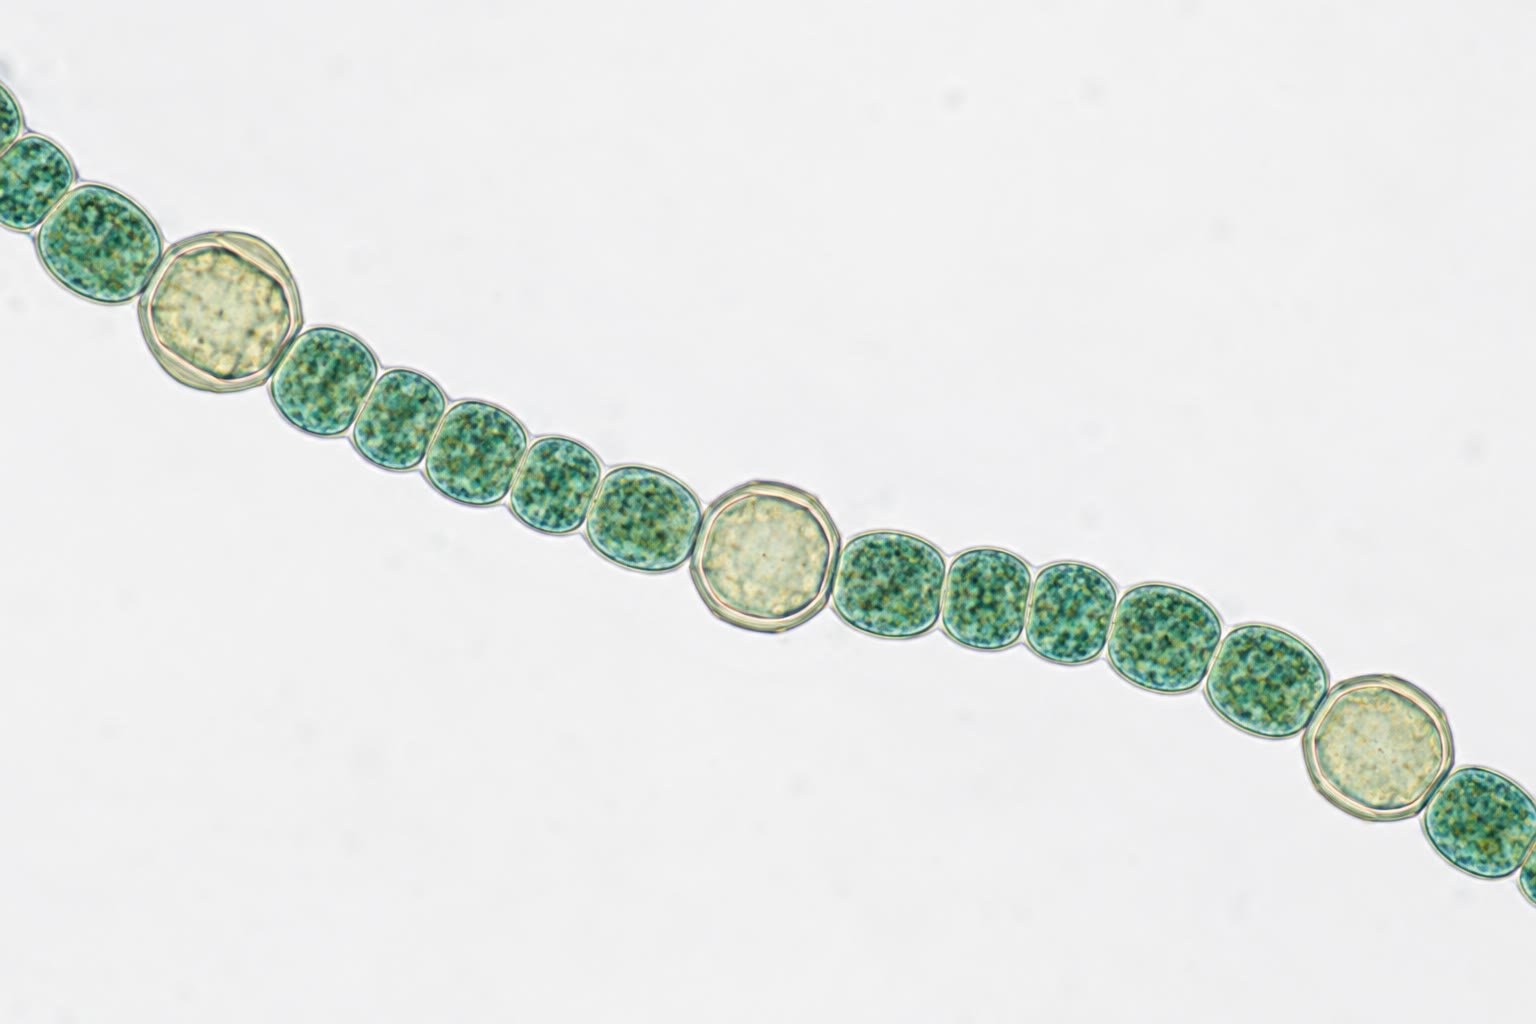
\includegraphics[width=0.62\linewidth]{images/book4/ai/b4-01-anabaena.jpg}

{\small Un filament d'\emph{Anabaena}~: une chaîne de cellules vertes
photosynthétiques interrompue par des hétérocystes plus gros et plus
pâles, les cellules qui fixent l'azote.}
\end{omfigure}

\begin{remark}[Dormance]\label{rem:b2:unicellular-diversity:spores}
Certains bâtonnets à Gram positif (\emph{Bacillus}, \emph{Clostridium})
répondent à la famine en construisant une \emph{endospore}~: une copie
du chromosome enveloppée de plusieurs tuniques déshydratées,
métaboliquement inerte, résistante à l'ébullition, aux rayonnements et à
des siècles de sécheresse, qui germe lorsque les conditions reviennent.
De nombreux \omterm{def:b2:unicellular-diversity:protist}{protistes} font de même avec un \emph{kyste}. La dormance est
l'autre manière de survivre à une mauvaise saison, à côté de la
motilité.
\end{remark}

\section{Les eucaryotes unicellulaires}

\begin{definition}[Les protistes~: un grade, non un groupe]\label{def:b2:unicellular-diversity:protist}
Les \emph{protistes}\index{protiste} sont les eucaryotes qui ne sont ni
des animaux, ni des plantes terrestres, ni des champignons --- pour la
plupart \omterm{def:b2:unicellular-diversity:unicellular}{unicellulaires}, certains coloniaux, quelques-uns (les laminaires)
\omterm{def:b2:unicellular-diversity:unicellular}{pluricellulaires}. Ils partagent la cellule eucaryote du volume de
première année (noyau, mitochondries, endomembranes, cytosquelette, cils
$9+2$) et rien d'autre en particulier~: les lignées qui les
contiennent sont aussi éloignées les unes des autres que les animaux le
sont des plantes. Les algues vertes se rangent avec les plantes
terrestres~; les diatomées et les algues brunes forment une lignée à
part~; les ciliés, les dinoflagellés et le parasite du paludisme en
forment une autre~; les amibes et les myxomycètes sont plus proches des
animaux et des champignons que de tous ceux-là. Le mot désigne un niveau
d'organisation --- la cellule eucaryote vivant seule --- et non une
branche de l'arbre.
\end{definition}

\begin{example}[Quatre manières d'être une cellule eucaryote isolée]\label{ex:b2:unicellular-diversity:four}
\emph{Chlamydomonas}~: une algue verte ovoïde à paroi glycoprotéique
dépourvue de cellulose, un chloroplaste unique en forme de coupe, un
stigma orangé qui fait de l'ombre à un photorécepteur pour que la
cellule sache de quel côté vient la lumière pendant qu'elle tourne, et
deux flagelles antérieurs qui battent à la manière d'une brasse~; c'est
un phototrophe. \emph{Paramecium}~: un cilié dont toute la surface bat
de cils en vagues coordonnées, un sillon oral en forme de bouche qui
balaie les bactéries vers des vacuoles digestives, deux \omterm{prop:b2:unicellular-diversity:osmoregulation}{vacuoles
contractiles} et deux sortes de noyaux --- un petit
\emph{micronucleus} germinal et un gros \emph{macronucleus}
fonctionnel qui porte des centaines de copies de chaque gène~; c'est un
phagotrophe. \emph{Amoeba}~: ni paroi ni forme fixe, elle se déplace et
se nourrit grâce à des \emph{pseudopodes} que la polymérisation de
l'actine pousse vers l'extérieur. La diatomée~: une cellule
photosynthétique enfermée dans deux valves de silice qui se recouvrent
comme une boîte et son couvercle, si finement ornées de pores que ces
coques servirent autrefois à tester les objectifs de microscope~; à la
division, chaque cellule fille garde une valve et en fabrique une
nouvelle, plus petite, à l'intérieur.
\end{example}

\begin{omfigure}
\begin{tikzpicture}[every node/.style={font=\scriptsize}]
  % Paramecium outline (slipper)
  \draw[thick, fill=omProp!8] plot[smooth cycle, tension=0.8] coordinates {(0,0) (1.5,0.9) (3.5,1.1) (5.5,0.7) (6.4,0) (5.5,-0.8) (3.5,-1.1) (1.5,-0.9)};
  % cilia
  \foreach \t in {3,9,...,357} {
    \pgfmathsetmacro{\cx}{3.2+3.25*cos(\t)}
    \pgfmathsetmacro{\cy}{1.08*sin(\t)}
    \pgfmathsetmacro{\dx}{3.2+3.55*cos(\t)}
    \pgfmathsetmacro{\dy}{1.32*sin(\t)}
    \draw[gray] (\cx,\cy) -- (\dx,\dy);
  }
  % macronucleus and micronucleus
  \draw[thick, fill=omDef!40] (3.2,0.05) ellipse (0.9 and 0.45);
  \fill[omDef!90!black] (2.4,0.55) circle (0.13);
  % oral groove and gullet
  \draw[thick, omThm] (4.3,-0.95) .. controls (3.6,-0.5) and (3.3,-0.2) .. (3.0,-0.35);
  \fill[omThm!30] (2.9,-0.45) circle (0.16);
  % food vacuoles
  \foreach \p in {(1.4,-0.3),(1.0,0.35),(4.8,0.35)} \draw[thick, omExo!80!black, fill=omExo!30] \p circle (0.17);
  % contractile vacuoles
  \foreach \c in {(1.2,0.0),(5.2,-0.2)} {
    \draw[thick, omDef] \c circle (0.28);
    \foreach \a in {0,60,...,300} \draw[omDef] \c ++(\a:0.28) -- ++(\a:0.22);
  }
  % labels
  \draw (2.4,0.55) -- (2.7,1.6) node[above] {micronucleus};
  \draw (3.6,0.3) -- (4.8,1.6) node[above] {macronucleus};
  \draw (1.2,0.28) -- (0.3,1.5) node[above, align=center] {vacuole contractile\\(avec canaux radiaires)};
  \draw (5.2,-0.48) -- (6.5,-1.5) node[below] {vacuole contractile};
  \draw (4.3,-0.95) -- (4.7,-1.75) node[below] {sillon oral};
  \draw (2.9,-0.61) -- (2.7,-1.6) node[below, align=center] {cytopharynx et vacuole\\digestive en formation};
  \draw (1.4,-0.47) -- (0.0,-1.5) node[below] {vacuoles digestives};
  \draw (6.35,0.4) -- (6.9,1.2) node[above, align=center] {cils};
\end{tikzpicture}

{\small \emph{Paramecium}, schéma~: le cortex cilié, les deux noyaux, le
sillon oral qui mène au cytopharynx où se forment les vacuoles
digestives, et les deux \omterm{prop:b2:unicellular-diversity:osmoregulation}{vacuoles contractiles} étoilées qui expulsent
l'eau que l'osmose fait entrer.}
\end{omfigure}

\begin{omfigure}
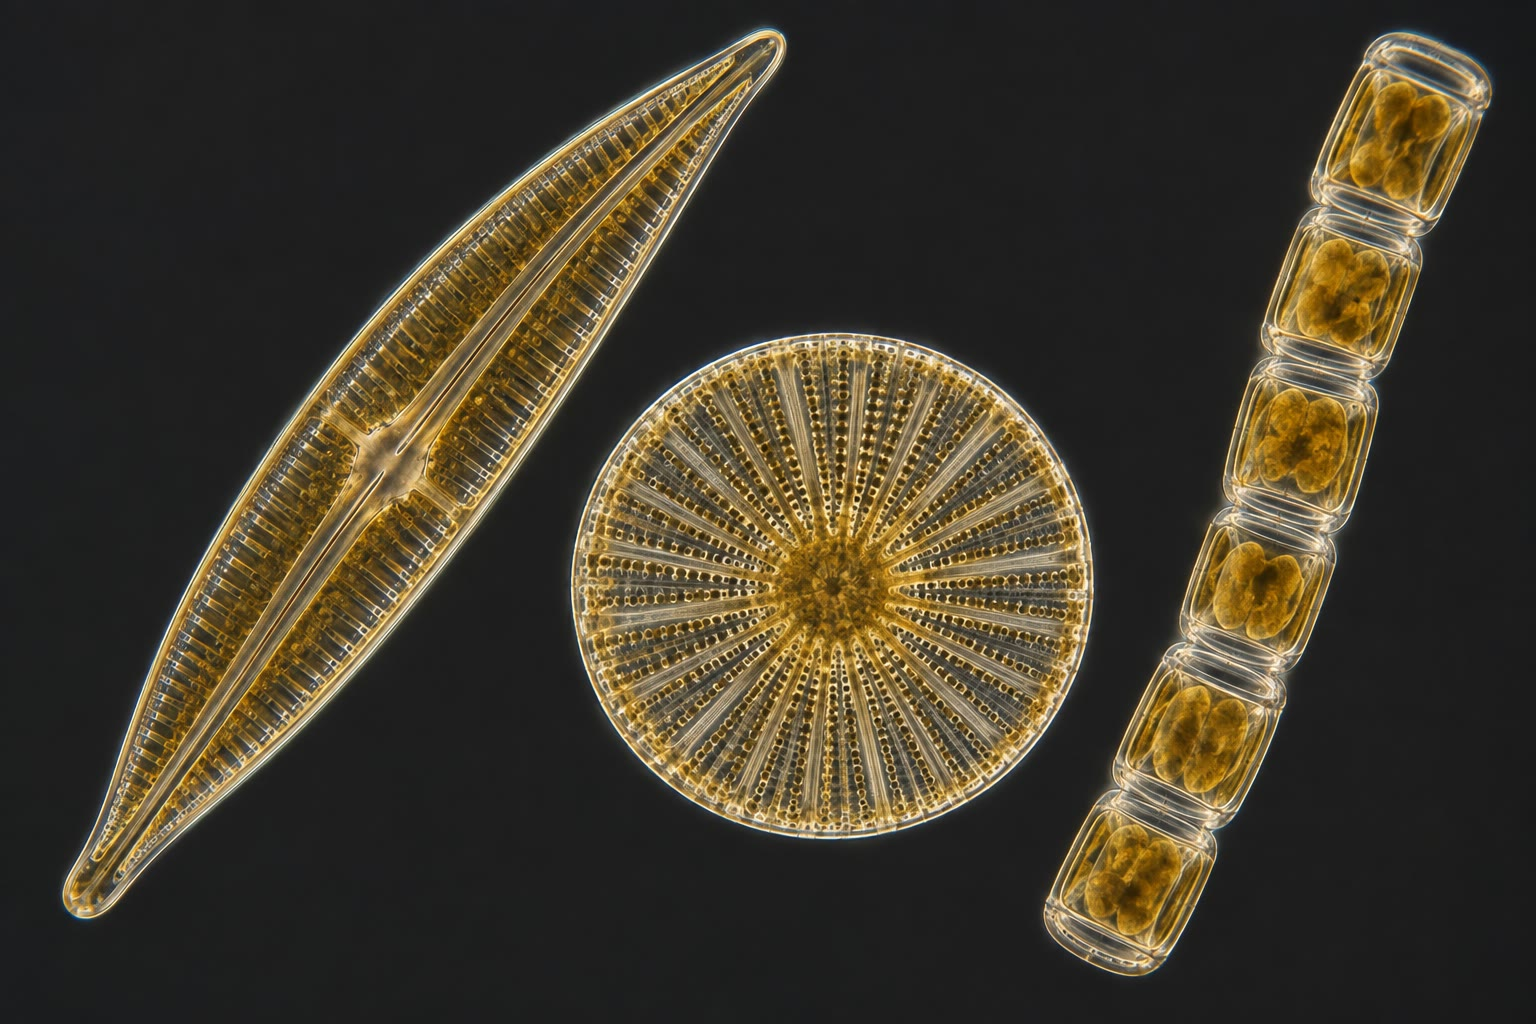
\includegraphics[width=0.6\linewidth]{images/book4/ai/b4-01-diatoms.jpg}

{\small Diatomées observées en microscopie à fond noir~: chaque cellule
vit dans une coque de silice à deux valves, percée de pores par
lesquels elle échange avec l'eau.}
\end{omfigure}

\begin{definition}[Modes de nutrition]\label{def:b2:unicellular-diversity:nutrition}
\index{phagotrophie}\index{osmotrophie}\index{mixotrophie}
Un eucaryote \omterm{def:b2:unicellular-diversity:unicellular}{unicellulaire} se nourrit de l'une de trois manières, ou de
deux à la fois. \emph{Phototrophie}~: il possède des chloroplastes et
fabrique sa propre matière organique à partir de la lumière et du
$\mathrm{CO_2}$ (algues vertes, diatomées, dinoflagellés).
\emph{Phagotrophie}~: il englobe des particules --- bactéries, autres
\omterm{def:b2:unicellular-diversity:protist}{protistes} --- dans une vacuole digestive où des enzymes lysosomales les
digèrent (amibes, ciliés, choanoflagellés). \emph{Osmotrophie}~: il
absorbe des molécules dissoutes à travers sa membrane, souvent après
avoir sécrété des enzymes à l'extérieur (levures, nombreux parasites).
Les \emph{mixotrophes} comme \emph{Euglena} font la photosynthèse à la
lumière et mangent à l'obscurité. Les \omterm{def:b2:unicellular-diversity:prokaryote}{procaryotes} ne peuvent pas
phagocyter~: la paroi l'interdit, et c'est pourquoi aucun \omterm{def:b2:unicellular-diversity:prokaryote}{procaryote}
n'est devenu prédateur par englobement.
\end{definition}

\begin{proposition}[L'osmorégulation en eau douce]\label{prop:b2:unicellular-diversity:osmoregulation}
\index{vacuole contractile}
Un \omterm{def:b2:unicellular-diversity:protist}{protiste} d'eau douce est bien plus salé à l'intérieur (quelque
\qty{100}{mmol/L} de solutés) que la mare (environ \qty{1}{mmol/L}), et
sa membrane laisse passer l'eau. L'eau entre donc en permanence par
osmose, à une vitesse proportionnelle à la surface et à la différence
de pression osmotique $\Delta\Pi = RT\,\Delta c$ --- environ
\qty{2.4}{bar} pour les valeurs ci-dessus. Une cellule pourvue d'une
paroi résiste par la turgescence~; une cellule nue gonflerait et
éclaterait en quelques minutes. La \emph{\omterm{prop:b2:unicellular-diversity:osmoregulation}{vacuole contractile}} est la
réponse~: un réservoir alimenté par des canaux radiaires, qui se remplit
d'eau pompée par des transporteurs couplés aux protons puis se
contracte en expulsant l'eau par un pore, toutes les quelques secondes à
toutes les quelques minutes. Une \emph{Paramecium} évacue son propre
volume d'eau toutes les demi-heures~; ses parents marins, dans un milieu
aussi salé qu'eux, n'ont aucune \omterm{prop:b2:unicellular-diversity:osmoregulation}{vacuole contractile}.
\end{proposition}

\section{La physique d'un petit nageur}

\begin{proposition}[La vie à faible nombre de Reynolds]\label{prop:b2:unicellular-diversity:reynolds}
\index{nombre de Reynolds}
Le \emph{\omterm{prop:b2:unicellular-diversity:reynolds}{nombre de Reynolds}} $Re = \rho v L/\eta$ compare les forces
d'inertie aux forces visqueuses pour un corps de taille $L$ se déplaçant
à la vitesse $v$ dans un fluide de masse volumique $\rho$ et de
viscosité $\eta$. Il vaut environ $10^6$ pour un nageur humain~; pour
\emph{Paramecium} (\qty{200}{\micro m}, \qty{1}{mm/s}) il vaut 0.2, et
pour une bactérie $10^{-5}$. En dessous de
$Re \approx 1$, l'inertie ne compte plus~: une cellule qui cesse de
battre s'arrête en moins d'un nanomètre, l'eau se comporte comme un
sirop épais, et un mouvement réciproque (le même geste en avant puis en
arrière) ne produit aucun déplacement net. Les petits nageurs utilisent
donc des mouvements non réciproques~: l'hélice tournante du flagelle
bactérien, le battement asymétrique d'un cil (coup efficace raide, coup
de retour replié), la brasse de \emph{Chlamydomonas}.
\end{proposition}

\begin{theorem}[Loi de Stokes et sédimentation]\label{thm:b2:unicellular-diversity:stokes}
\index{loi de Stokes}
Une sphère de rayon $r$ et de masse volumique $\rho_{\text{cellule}}$ qui
se déplace lentement dans un fluide de viscosité $\eta$ subit une
traînée $F = 6\pi\eta r v$. Livrée à elle-même dans une eau de masse
volumique $\rho$, elle coule à la vitesse limite
\[
v_s = \frac{2\,r^2\,(\rho_{\text{cellule}} - \rho)\,g}{9\eta},
\]
proportionnelle au carré de son rayon~: une cellule dix fois plus grande
coule cent fois plus vite. C'est pourquoi le phytoplancton est petit,
pourquoi les diatomées portent des épines et des gouttelettes d'huile,
et pourquoi une \emph{Chlamydomonas} qui cesse de nager sort de la zone
éclairée en quelques jours.
\end{theorem}
\begin{proof}
À la vitesse limite, la traînée équilibre le poids apparent (le poids
diminué de la poussée d'Archimède)~: $6\pi\eta r v_s = \tfrac{4}{3}\pi r^3
(\rho_{\text{cellule}} - \rho) g$. En résolvant pour $v_s$, on obtient la
formule. La loi de traînée elle-même est établie dans la série de
physique pour $Re \ll 1$~; on l'admet ici.
\end{proof}

\begin{example}[La chute d'une diatomée]\label{ex:b2:unicellular-diversity:fall}
Une diatomée centrique de rayon \qty{10}{\micro m}, plus dense que l'eau
de mer de \qty{100}{kg/m^3} ($\eta = \qty{1e-3}{Pa.s}$), coule à
$v_s = 2\times 10^{-10}\times 100\times 9.81/(9\times 10^{-3}) =
\qty{2.2e-5}{m/s}$, soit environ \qty{2}{m} par jour~: elle quitterait
la couche éclairée de \qty{50}{m} en moins d'un mois. Ses populations
survivent parce que la turbulence brasse l'eau, parce que les
gouttelettes d'huile et une faible densité réduisent
$\rho_{\text{cellule}} - \rho$, et parce qu'une cellule qui coule en se
divisant en chemin laisse des descendants qui sont remontés à leur tour.
\end{example}

\begin{omfigure}
\begin{tikzpicture}
\begin{axis}[
  width=0.8\linewidth, height=6.0cm,
  axis x line=bottom, axis y line=left,
  xmode=log, ymode=log,
  xmin=0.5, xmax=200, ymin=1e-3, ymax=1e4,
  xlabel={rayon (\unit{\micro m})}, ylabel={vitesse de sédimentation (\unit{\micro m/s})},
  xlabel style={font=\small, at={(axis description cs:0.5,-0.1)}, anchor=north},
  ylabel style={font=\small},
  tick label style={font=\small},
  clip=false,
]
\addplot[very thick, omDef, domain=0.5:200, samples=40] {0.218*x^2};
\addplot[only marks, mark=*, mark size=1.8pt, omThm] coordinates {(1,0.218) (10,21.8) (100,2180)};
\node[font=\scriptsize, anchor=west] at (axis cs:1.15,0.218) {bactérie};
\node[font=\scriptsize, anchor=west] at (axis cs:11.5,21.8) {diatomée};
\node[font=\scriptsize, anchor=east] at (axis cs:85,2180) {grand protiste};
\end{axis}
\end{tikzpicture}

{\small Vitesse de sédimentation de Stokes en fonction du rayon, pour
des cellules plus denses que l'eau de \qty{100}{kg/m^3}. La pente de 2
en axes logarithmiques traduit la loi en $r^2$~: une bactérie coule
d'un centimètre par jour, un grand \omterm{def:b2:unicellular-diversity:protist}{protiste} de deux ou trois mètres par
heure.}
\end{omfigure}

\section{Reproduction et sexualité dans une seule cellule}

\begin{definition}[Modes de division]\label{def:b2:unicellular-diversity:division}
\index{division binaire}\index{bourgeonnement}\index{division multiple}
Un \omterm{def:b2:unicellular-diversity:unicellular}{organisme unicellulaire} se reproduit en se divisant. \emph{Division
binaire}~: la cellule double de taille et se scinde en deux cellules
filles égales (bactéries, \emph{Paramecium}, \emph{Amoeba}).
\emph{Bourgeonnement}~: une petite cellule fille pousse hors de la
cellule mère puis s'en détache (levure~; la mère garde une cicatrice et
peut bourgeonner une vingtaine de fois). \emph{Division multiple}~: la
cellule devient grande, puis se divise plusieurs fois de suite
rapidement à l'intérieur de la paroi maternelle et libère 4, 8, 16
cellules filles ou plus à la fois (\emph{Chlamydomonas}, le parasite du
paludisme dans une hématie). En conditions constantes, le nombre de
cellules croît exponentiellement, $N(t) = N_0\,2^{t/T}$, où $T$ est le
\emph{temps de génération}\index{temps de generation@temps de génération}~: vingt minutes pour
\emph{E.~coli} en milieu riche, un jour pour de nombreuses algues, une
semaine pour certains ciliés. (La croissance en fonction de la
nourriture est traitée au \cref{ch:b2:microbial-metabolism}.)
\end{definition}

\begin{proposition}[Sexualité sans reproduction~: la conjugaison chez \emph{Paramecium}]\label{prop:b2:unicellular-diversity:conjugation}
\index{conjugaison!cilies@ciliés}
Deux \emph{Paramecium} de types sexuels complémentaires s'accolent par
leurs faces orales. Dans chacune, le micronucleus diploïde subit la
méiose et donne quatre noyaux haploïdes, dont trois dégénèrent~; le
survivant se divise par mitose en un noyau stationnaire et un noyau
migrateur, et les deux cellules échangent leurs noyaux migrateurs à
travers la jonction. Chaque cellule fusionne ensuite son noyau
stationnaire avec celui qu'elle a reçu, et les deux partenaires se
séparent, chacun avec un nouveau micronucleus diploïde de même génotype
que celui de son partenaire. L'ancien macronucleus se désagrège et un
nouveau est construit à partir du nouveau micronucleus. Aucune cellule
nouvelle n'a été produite~: la conjugaison est un brassage génétique ---
méiose et fécondation, \cref{ch:b2:meiosis-heredity} --- découplé de la
multiplication. La conjugaison bactérienne, qui transfère un \omterm{def:b2:unicellular-diversity:prokaryote}{plasmide}
dans un seul sens, d'un donneur à un receveur, est un processus
différent qui porte le même nom
(\cref{ch:b2:genome-diversification}).
\end{proposition}

\begin{omfigure}
\begin{tikzpicture}[every node/.style={font=\scriptsize}]
  \foreach \i/\x in {0/0,1/3.6,2/7.2,3/10.8} {
    \draw[thick, fill=omProp!8] (\x,0.55) ellipse (1.0 and 0.5);
    \draw[thick, fill=omProp!8] (\x,-0.55) ellipse (1.0 and 0.5);
  }
  % stage 0: two cells, diploid micronuclei 2n
  \fill[omDef!90!black] (0,0.55) circle (0.12); \node[right] at (0.15,0.55) {$2n$};
  \fill[omDef!90!black] (0,-0.55) circle (0.12); \node[right] at (0.15,-0.55) {$2n$};
  \node[below, align=center] at (0,-1.15) {deux cellules s'accolent};
  % stage 1: meiosis, 4 haploid, 3 degenerate
  \foreach \dy in {0.55,-0.55} {
    \fill[omDef!90!black] (3.6-0.3,\dy+0.15) circle (0.08);
    \fill[gray!60] (3.6+0.1,\dy+0.2) circle (0.06);
    \fill[gray!60] (3.6+0.3,\dy-0.05) circle (0.06);
    \fill[gray!60] (3.6-0.1,\dy-0.25) circle (0.06);
  }
  \node[below, align=center] at (3.6,-1.15) {méiose~:\\4 noyaux haploïdes,\\trois dégénèrent};
  % stage 2: mitosis, exchange
  \foreach \dy in {0.55,-0.55} {
    \fill[omDef!90!black] (7.2-0.35,\dy) circle (0.08);
    \fill[omThm] (7.2+0.35,\dy) circle (0.08);
  }
  \draw[->, thick, omThm] (7.55,0.45) -- (7.55,-0.45);
  \draw[->, thick, omThm] (6.85,-0.45) -- (6.85,0.45);
  \node[below, align=center] at (7.2,-1.15) {mitose~; les noyaux\\migrateurs (en rouge)\\sont échangés};
  % stage 3: fusion 2n
  \fill[omDef!90!black] (10.8,0.55) circle (0.12); \node[right] at (10.95,0.55) {$2n$};
  \fill[omDef!90!black] (10.8,-0.55) circle (0.12); \node[right] at (10.95,-0.55) {$2n$};
  \node[below, align=center] at (10.8,-1.15) {fécondation~:\\nouveaux noyaux diploïdes\\identiques~; les cellules se séparent};
  \foreach \x in {1.3,4.9,8.5} \draw[->, thick, gray] (\x,0) -- (\x+1.0,0);
\end{tikzpicture}

{\small La conjugaison chez \emph{Paramecium}. Deux cellules échangent
des noyaux haploïdes puis se séparent, chacune portant un micronucleus
diploïde recombiné~; le nombre de cellules n'a pas changé.}
\end{omfigure}

\section{Vers la pluricellularité}

\begin{proposition}[La série des volvocales]\label{prop:b2:unicellular-diversity:volvox}
\index{Volvox@\emph{Volvox}}\index{pluricellularite, origine de la@pluricellularité, origine de la}
Chez les algues vertes, une lignée montre, parmi ses espèces actuelles,
les étapes qui mènent d'une cellule à un corps. \emph{Chlamydomonas} vit
seule. \emph{Gonium} est une plaque de 4 à 16 cellules identiques qui
nagent ensemble. \emph{Pandorina} et \emph{Eudorina} sont des sphères
creuses de 16 à 32 cellules, encore toutes semblables, chacune capable
de fonder une nouvelle colonie. \emph{Pleodorina} possède quelques
petites cellules qui ne font que nager et ne se divisent jamais.
\emph{Volvox} est une sphère de \num{500} à \num{50000} petites cellules
somatiques, flagellées, qui mourront avec la colonie, autour d'une
poignée de grandes cellules germinales (les gonidies) qui se divisent
pour former des sphères filles à l'intérieur de la mère. Cellules
somatiques et cellules germinales sont apparues~: c'est le seuil de la
pluricellularité, franchi dans cette lignée il y a quelque \num{200}
millions d'années et, indépendamment, au moins vingt-cinq fois ailleurs
dans l'arbre du vivant --- chez les animaux, les plantes, les
champignons, les algues brunes, les algues rouges et plusieurs groupes
bactériens.
\end{proposition}
\begin{proof}[Faits expérimentaux]
La phylogénie moléculaire des volvocales, construite à partir de
dizaines de gènes, place \emph{Chlamydomonas} à la base et \emph{Volvox}
aux extrémités, les formes \omterm{def:b2:unicellular-diversity:unicellular}{coloniales} entre les deux et le nombre de
cellules augmentant le long des branches~; le génome de \emph{Volvox
carteri} (2010) ne diffère de celui de \emph{Chlamydomonas} que par
quelques centaines de gènes, principalement ceux de la matrice
extracellulaire qui retient les cellules et ceux des régulateurs qui
répriment la division dans les cellules somatiques. La transition a
demandé remarquablement peu de matériel génétique nouveau.
\end{proof}

\begin{omfigure}
\begin{tikzpicture}[every node/.style={font=\scriptsize}]
  % Chlamydomonas
  \draw[thick, fill=omProp!25] (0,0) circle (0.22);
  \node[below=0.35cm, align=center] at (0,0) {\emph{Chlamydomonas}\\1 cellule};
  % Gonium plate
  \begin{scope}[xshift=2.2cm]
    \foreach \x in {-0.3,0,0.3} \foreach \y in {-0.3,0,0.3} \draw[thick, fill=omProp!25] (\x,\y) circle (0.14);
    \draw[gray, dashed] (-0.55,-0.55) rectangle (0.55,0.55);
    \node[below=0.7cm, align=center] at (0,0) {\emph{Gonium}\\plaque de 8--16};
  \end{scope}
  % Eudorina ball
  \begin{scope}[xshift=4.5cm]
    \draw[gray, dashed] (0,0) circle (0.6);
    \foreach \a in {0,45,...,315} \draw[thick, fill=omProp!25] (\a:0.55) circle (0.13);
    \draw[thick, fill=omProp!25] (0,0.1) circle (0.13);
    \node[below=0.7cm, align=center] at (0,0) {\emph{Eudorina}\\sphère de 32,\\toutes semblables};
  \end{scope}
  % Pleodorina
  \begin{scope}[xshift=7.4cm]
    \draw[gray, dashed] (0,0) circle (0.7);
    \foreach \a in {0,30,...,330} \draw[thick, fill=omProp!25] (\a:0.62) circle (0.09);
    \foreach \a in {60,180,300} \draw[thick, fill=omProp!60] (\a:0.62) circle (0.14);
    \node[below=0.8cm, align=center] at (0,0) {\emph{Pleodorina}\\certaines cellules\\ne font que nager};
  \end{scope}
  % Volvox
  \begin{scope}[xshift=10.6cm]
    \draw[thick, fill=omProp!6] (0,0) circle (0.95);
    \foreach \a in {0,12,...,348} \fill[omProp!70] (\a:0.9) circle (0.035);
    \foreach \a in {0,12,...,348} \fill[omProp!50] (\a:0.72) circle (0.03);
    \foreach \p in {(0.25,0.2),(-0.3,-0.25),(0.1,-0.4),(-0.2,0.35)} \draw[thick, omThm, fill=omThm!40] \p circle (0.13);
    \node[below=1.05cm, align=center] at (0,0) {\emph{Volvox}\\des milliers de cellules somatiques\\et quelques cellules germinales (en rouge)};
  \end{scope}
  \foreach \x in {0.5,3.0,5.3,8.3} \draw[->, gray] (\x,0) -- (\x+0.6,0);
\end{tikzpicture}

{\small La série des volvocales~: une cellule isolée, une plaque, une
sphère creuse de cellules identiques, une sphère dont certaines cellules
ont renoncé à se diviser, et \emph{Volvox}, où des milliers de cellules
somatiques mortelles entourent quelques cellules germinales.}
\end{omfigure}

\begin{omfigure}
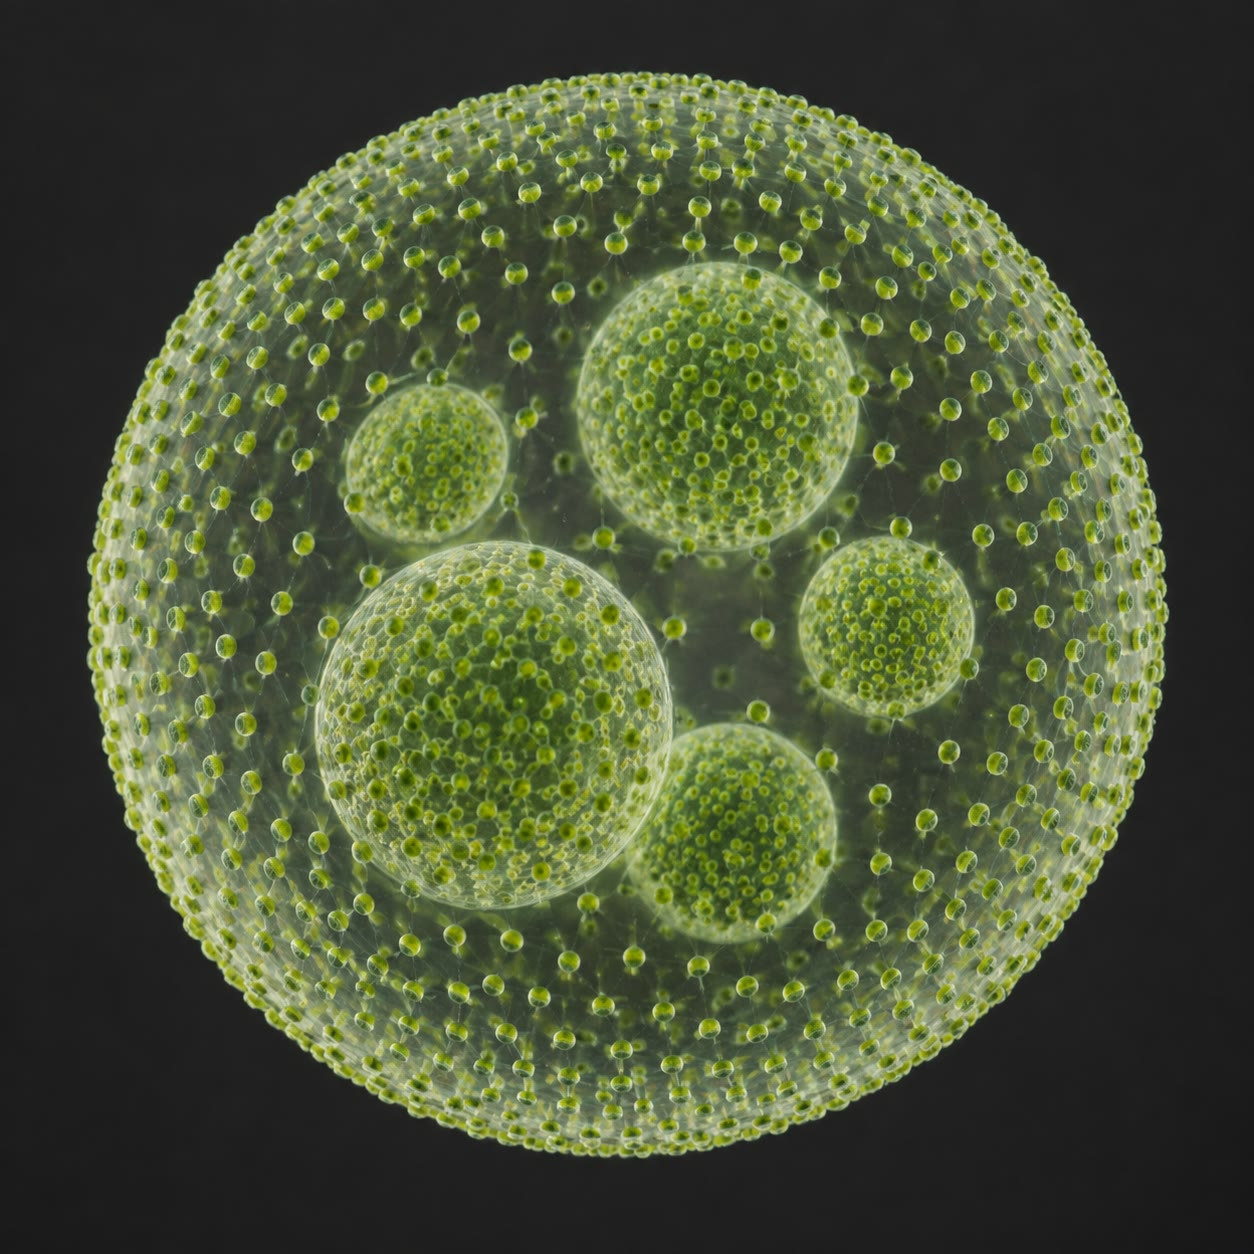
\includegraphics[width=0.55\linewidth]{images/book4/ai/b4-01-volvox.jpg}

{\small Une colonie de \emph{Volvox}~: une sphère verte et creuse de
cellules flagellées, abritant des colonies filles en croissance.}
\end{omfigure}

\begin{remark}[Pourquoi diviser le travail~?]\label{rem:b2:unicellular-diversity:whydivide}
Chez ces algues, une cellule ne peut pas nager et se diviser en même
temps~: les corps basaux qui ancrent les flagelles sont nécessaires à
l'organisation du fuseau. Une cellule isolée alterne~; une petite
colonie peut se permettre de cesser de nager pendant que toutes ses
cellules se divisent~; une grande colonie sortirait de la zone éclairée
(\omterm{thm:b2:unicellular-diversity:stokes}{loi de Stokes}, \cref{thm:b2:unicellular-diversity:stokes}) pendant
les heures que dure sa division. Au-delà d'une certaine taille, garder
certaines cellules en train de nager pendant que d'autres se divisent
vaut la perte de leur descendance --- et un soma naît. Les
choanoflagellés, flagellés à collerette dont la cellule est une copie
de la cellule nourricière des éponges, montrent les mêmes premiers pas
sur la branche qui a mené aux animaux.
\end{remark}

\section{Exercices}

\begin{exercise}[$\star$]\label{exo:b2:unicellular-diversity:1}
Définir \omterm{def:b2:unicellular-diversity:unicellular}{unicellulaire}, \omterm{def:b2:unicellular-diversity:unicellular}{colonial} et \omterm{def:b2:unicellular-diversity:unicellular}{pluricellulaire}, et ranger
\emph{E.~coli}, \emph{Gonium}, \emph{Volvox} et une cellule de levure
dans la bonne catégorie en justifiant.
\end{exercise}

\begin{exercise}[$\star$]\label{exo:b2:unicellular-diversity:2}
Calculer le \omterm{prop:b2:unicellular-diversity:surface}{rapport surface/volume} d'un coque de rayon
\qty{0.5}{\micro m} et d'un \omterm{def:b2:unicellular-diversity:protist}{protiste} sphérique de rayon
\qty{50}{\micro m}. Lequel respire le plus vite par unité de
cytoplasme, et pourquoi~?
\end{exercise}

\begin{exercise}[$\star$]\label{exo:b2:unicellular-diversity:3}
Donner trois différences structurales entre une bactérie et un
eucaryote \omterm{def:b2:unicellular-diversity:unicellular}{unicellulaire}, et une chose qu'une amibe peut faire et
qu'une bactérie ne peut pas faire.
\end{exercise}

\begin{exercise}[$\star$]\label{exo:b2:unicellular-diversity:4}
Indiquer la fonction de chacune des structures suivantes de
\emph{Paramecium}~: cils, sillon oral, vacuole digestive, \omterm{prop:b2:unicellular-diversity:osmoregulation}{vacuole
contractile}, macronucleus, micronucleus.
\end{exercise}

\begin{exercise}[$\star\star$]\label{exo:b2:unicellular-diversity:5}
Avec $D = \qty{5e-10}{m^2/s}$ pour un métabolite dans le cytoplasme,
combien de temps la diffusion met-elle pour traverser une bactérie de
\qty{1}{\micro m} et une amibe de \qty{500}{\micro m}~? Commenter ce que
l'amibe doit faire et dont la bactérie peut se passer.
\end{exercise}

\begin{exercise}[$\star\star$]\label{exo:b2:unicellular-diversity:6}
Calculer le \omterm{prop:b2:unicellular-diversity:reynolds}{nombre de Reynolds} d'une \emph{Paramecium}
(\qty{200}{\micro m}, \qty{1}{mm/s}), d'une bactérie (\qty{2}{\micro m},
\qty{20}{\micro m/s}) et d'un nageur humain (\qty{2}{m}, \qty{1}{m/s}),
avec $\rho = \qty{1000}{kg/m^3}$ et $\eta = \qty{1e-3}{Pa.s}$. Pourquoi
un nageur peut-il glisser après un mouvement de bras alors qu'une
bactérie ne le peut pas~?
\end{exercise}

\begin{exercise}[$\star\star$]\label{exo:b2:unicellular-diversity:7}
Une diatomée de rayon \qty{10}{\micro m} est plus dense que l'eau de
\qty{100}{kg/m^3}. Calculer sa vitesse de sédimentation et le temps
qu'elle met à descendre de \qty{50}{m}. De quel facteur ce temps
change-t-il si la cellule divise son rayon par deux~? Si elle réduit
son excès de masse volumique à \qty{20}{kg/m^3}~?
\end{exercise}

\begin{exercise}[$\star\star$]\label{exo:b2:unicellular-diversity:8}
On modélise une \emph{Paramecium} par un ellipsoïde de demi-axes
\num{100}, \num{25} et \qty{25}{\micro m} ($V = \tfrac{4}{3}\pi abc$).
Elle expulse son propre volume d'eau toutes les \qty{30}{min}. Calculer
le flux entrant d'eau en \unit{\micro m^3/s} et en litres par seconde.
\end{exercise}

\begin{exercise}[$\star\star$]\label{exo:b2:unicellular-diversity:9}
La concentration d'un attractant double sur \qty{1}{mm}. Quelle est la
différence relative entre les deux extrémités d'une bactérie de
\qty{1}{\micro m}~? Entre le début et la fin d'une course de \qty{1}{s}
à \qty{20}{\micro m/s}~? Le dénombrement de $N$ molécules comporte une
erreur relative d'environ $1/\sqrt{N}$~: expliquer pourquoi la bactérie
compare des instants plutôt que des côtés.
\end{exercise}

\begin{exercise}[$\star\star\star$]\label{exo:b2:unicellular-diversity:10}
\emph{Thiomargarita namibiensis} est une bactérie sulfureuse sphérique
de \qty{500}{\micro m} de diamètre dont le cytoplasme forme une couche
de \qty{2}{\micro m} d'épaisseur autour d'une vacuole de nitrate.
Calculer le rapport de sa surface à son volume \emph{cytoplasmique} et
le comparer à celui d'\emph{E.~coli} (un cylindre de rayon
\qty{0.5}{\micro m}~; négliger les extrémités). Expliquer comment la
vacuole lui permet d'être si grande, et à quoi sert le nitrate.
\end{exercise}

\begin{exercise}[$\star\star\star$]\label{exo:b2:unicellular-diversity:11}
Chez \emph{Volvox}, les cellules somatiques ne se divisent jamais et
meurent avec la colonie. À l'aide de la contrainte liée aux flagelles et
de la \omterm{thm:b2:unicellular-diversity:stokes}{loi de Stokes}, expliquer pourquoi de telles cellules sont
avantageuses dans une colonie de \num{10000} cellules mais pas dans une
colonie de 16, et pourquoi les cellules germinales sont les plus
grandes cellules de la sphère.
\end{exercise}

\begin{exercise}[$\star\star\star$]\label{exo:b2:unicellular-diversity:12}
«~Les \omterm{def:b2:unicellular-diversity:protist}{protistes} forment un grade, non un clade.~» Expliquer la
distinction à l'aide des lignées nommées dans ce chapitre, et dire
pourquoi la même affirmation est vraie des «~\omterm{def:b2:unicellular-diversity:prokaryote}{procaryotes}~» et fausse
des «~cyanobactéries~».
\end{exercise}

\section{Problème~: une goutte d'eau de mare}

\begin{problem}[{Problème du week-end --- un échantillon d'eau de mare est
dénombré, mis en culture et analysé du point de vue de la physique qui
gouverne ses cellules, jusqu'au bilan d'eau et d'énergie d'une algue verte}]
\label{pb:b2:unicellular-diversity:1}
On prélève au printemps un échantillon d'une mare de \qty{1000}{m^3}.
Sous le microscope, une cellule de comptage dont la grille couvre
\qty{1}{mm}$\times$\qty{1}{mm}, sous une lamelle maintenue
\qty{0.1}{mm} au-dessus, montre 24 cellules de \emph{Chlamydomonas}
(sphères de rayon \qty{5}{\micro m}, de masse volumique
\qty{1050}{kg/m^3}). On prendra $\rho = \qty{1000}{kg/m^3}$,
$\eta = \qty{1e-3}{Pa.s}$, $g = \qty{9.81}{m/s^2}$, $R =
\qty{8.314}{J/mol/K}$, $T = \qty{293}{K}$, $D = \qty{1.9e-9}{m^2/s}$
pour le $\mathrm{CO_2}$ dans l'eau.

\medskip
\noindent\textbf{Partie I --- Dénombrement.}
\begin{enumerate}
  \item Calculer le volume d'eau situé sous la grille, en microlitres.
  \item En déduire la densité de \emph{Chlamydomonas} dans la mare, en
        cellules par millilitre.
  \item Calculer le volume et le \omterm{prop:b2:unicellular-diversity:surface}{rapport surface/volume} d'une cellule.
  \item Quelle fraction du volume d'eau de la mare ces cellules
        occupent-elles~?
  \item Combien de \emph{Chlamydomonas} la mare contient-elle~?
  \item Une cyanobactérie filamenteuse est également présente. Donner
        deux caractéristiques visibles au microscope qui la distinguent
        de l'algue.
\end{enumerate}

\medskip
\noindent\textbf{Partie II --- Croissance.}
L'échantillon est gardé à la lumière et dénombré de nouveau au bout de
\qty{48}{h}~: \num{384} cellules sous la grille.
\begin{enumerate}[resume]
  \item Calculer le \omterm{def:b2:unicellular-diversity:division}{temps de génération} $T$.
  \item Calculer la constante de croissance $k$ dans $N = N_0 e^{kt}$,
        en \unit{h^{-1}}.
  \item Combien de temps faudrait-il à la population de la mare pour
        atteindre \qty{1e8}{} cellules par millilitre à ce rythme~?
  \item Donner trois raisons pour lesquelles elle n'y parviendra pas.
  \item Si les cellules ne croissent que pendant les \qty{12}{h} de jour
        et pas du tout la nuit, combien de temps la même augmentation
        prend-elle~?
  \item \emph{Chlamydomonas} se divise par \omterm{def:b2:unicellular-diversity:division}{division multiple} et libère
        4, 8 ou 16 cellules filles à la fois. Expliquer pourquoi le
        dénombrement définit néanmoins bien un \omterm{def:b2:unicellular-diversity:division}{temps de génération}.
\end{enumerate}

\medskip
\noindent\textbf{Partie III --- La physique de la cellule.}
\begin{enumerate}[resume]
  \item Calculer le \omterm{prop:b2:unicellular-diversity:reynolds}{nombre de Reynolds} d'une cellule qui nage à
        \qty{100}{\micro m/s}.
  \item Une cellule de masse $m$ qui cesse de battre des flagelles
        parcourt sur son élan une distance $mv/(6\pi\eta r)$. La
        calculer.
  \item Calculer la vitesse de sédimentation d'une cellule qui a cessé
        de nager.
  \item Comparer le temps mis pour couler de \qty{1}{m} au temps mis
        pour remonter de \qty{1}{m} à la nage.
  \item La mare contient \qty{10}{\micro mol/L} de $\mathrm{CO_2}$
        dissous. Calculer l'apport diffusif maximal de
        $\mathrm{CO_2}$ à une cellule, en molécules par seconde.
  \item Une cellule contient \qty{100}{pg} de carbone et double cette
        quantité en une génération. Calculer sa demande moyenne en
        carbone, en molécules par seconde, et le rapport de l'apport à la
        demande.
  \item Refaire la comparaison pour une cellule hypothétique de rayon
        \qty{50}{\micro m} de même densité en carbone. Conclure.
\end{enumerate}

\medskip
\noindent\textbf{Partie IV --- Eau et énergie.}
Le cytoplasme contient \qty{100}{mmol/L} de solutés, la mare
\qty{1}{mmol/L}. La conductivité hydraulique de la membrane est $L_p =
\qty{1e-14}{m.s^{-1}.Pa^{-1}}$ (flux volumique d'eau par unité de
surface et par unité de différence de pression). L'hydrolyse d'un ATP
fournit \qty{50}{kJ/mol}~; la fixation d'un atome de carbone coûte
trois ATP.
\begin{enumerate}[resume]
  \item Calculer la différence de pression osmotique de part et d'autre
        de la membrane.
  \item Calculer le volume d'eau qui entre dans la cellule par seconde,
        en \unit{\micro m^3/s}.
  \item Sans \omterm{prop:b2:unicellular-diversity:osmoregulation}{vacuole contractile}, combien de temps la cellule
        mettrait-elle à doubler de volume~?
  \item Calculer la puissance minimale nécessaire pour expulser cette
        eau contre la pression osmotique.
  \item La convertir en molécules d'ATP par seconde et la comparer à
        l'ATP que la cellule consacre à la fixation du carbone
        (question 18).
  \item Énoncer le résultat~: le flux d'eau entrant dans la cellule, le
        temps qu'elle mettrait à éclater, et la fraction de son énergie
        que coûte le maintien de son équilibre hydrique.
\end{enumerate}
\end{problem}
